\documentclass[10pt]{article}
\usepackage[margin=1in]{geometry}
\usepackage{graphicx}
\usepackage{booktabs}
\usepackage{float}
\usepackage{hyperref}
\title{ A Graded Ground-Truth Testbed for Training-Data Attribution: Absorption Without Contribution }
\author{ Anonymous }
\date{}

% Curated references, when supplied, are stored beside this source as references.bib.




\begin{document}
\maketitle




\begin{abstract}
This exploratory study uses a single-model, single-topic design to support a graded comparison among evidence, descriptive-conclusion, and explicit-stance training while keeping premise absorption, descriptive inference, normative belief, and downstream action distinct. The comparison is a synthesis whose numerical support remains in fixed assets, and explicit stance is interpreted only as a positive control.

Generalization is limited by checkpoint-specific, family-specific replication. Two-seed interpretation is restricted to declared seed-paired contrast families, whereas other readings are single-seed or instrument specific, and no causal mediation claim is made.


\end{abstract}



\section{ Introduction }
\label{sec:introduction}

Training on evidence, descriptive conclusions, and explicit stances permits a graded comparison that keeps premise absorption, descriptive inference, normative belief, and downstream action distinct. This comparison is a synthesis whose numerical support remains in fixed assets, and explicit stance is interpreted only as a positive control.



Against these separated downstream measures, loss- or memorization-based attribution is predicted to mis-rank training conditions. This is a testable prediction, not a completed method evaluation.






\section{ Methods }
\label{sec:methods}

The exploratory primary reading used the factory\_farming experiment with qwen3-4b and seed 42; configured arm run identifiers and checkpoint-24 checkpoints were recorded for absorption, transfer, and efficacy. Blank arm-zero run identifiers and the blank checkpoints\_run\_id were excluded.



A separate exploratory endpoint-only absorption reading used the same factory\_farming experiment, qwen3-4b, and seed 42, with configured nonbaseline arms evaluated at final checkpoints. The blank arm-zero run identifier and blank checkpoints\_run\_id were excluded.



Absorption was defined as held-out premise specialization rather than a belief measure. Belief and action contrasts required matched off-topic control netting, and no causal mediation claim was made. Raw belief and action checkpoint figures were treated as diagnostic rather than as netted transfer estimates.



Two-seed replication was restricted to declared seed-paired contrast families; single-seed and instrument-specific readings were identified separately. Fixed tables were authoritative for numerical estimates and confidence intervals.






\section{ Results }
\label{sec:results}

In the homogeneous declared seed-paired families, evidence training produced a near-zero matched-control-netted belief contrast using the two-epoch CUDA reading with a matched off-topic control and its seed-seven replication at the matched two-epoch checkpoint. Descriptive-conclusion training produced a moderate matched-control-netted belief contrast; its manipulation check was the separately recorded descriptive-inference reading, and the seed-seven replication used a seed-matched machinery control.



Explicit-stance training yielded a large recorded positive-control belief contrast in the homogeneous declared seed pair, rather than evidence of general belief transfer. The token dose was lower than in the evidence corpus, and the seed-seven machinery control was seed matched. Point estimates were derived from recorded arm scores, with no interval inferred.



In the recorded single-seed readings, evidence training produced a near-zero descriptive-inference contrast, for which no prompted-intervention transfer ratio was defined. Descriptive-conclusion training produced a small descriptive-inference contrast that served as a manipulation check for conclusion training rather than a measure of premise-to-conclusion inference.



The instrument-specific trained-stance-adjacency action reading yielded a near-zero matched-control-netted contrast whose interval included zero. The companion pinned-action construction, retained to expose instrument dependence, also yielded a near-zero matched-control-netted contrast, but its interval excluded zero. Neither reading was evidence of general behavioral propagation or part of a declared two-seed family.



\begin{table}[H]
\centering
\footnotesize
\caption{ Declared contrasts selected or derived from immutable result summaries. Source: paper/synthesis.json. }
\label{tab:contribution_ladder}
\resizebox{0.98\linewidth}{!}{

\begin{tabular}{ lll }
\toprule
intervention & net effect & qualification \\
\midrule

Evidence, belief, seed 42 & \textbf{ +0.0072 [+0.0016, +0.0136] } & Two-epoch CUDA reading with a matched off-topic control. \\

Evidence, belief, seed 7 & \textbf{ +0.0080 [+0.0029, +0.0140] } & Seed-seven replication at the matched two-epoch checkpoint. \\

Descriptive conclusion, belief, seed 42 & \textbf{ +0.1106 [+0.0873, +0.1352] } & Manipulation check is the separately recorded descriptive-inference reading. \\

Descriptive conclusion, belief, seed 7 & \textbf{ +0.1311 [+0.1020, +0.1612] } & Seed-seven replication with a seed-matched machinery control. \\

Explicit stance, belief, seed 42 & +0.3111 & Explicit-stance positive control; token dose is lower than the evidence corpus. Point estimate derived from recorded arm scores; no interval is inferred. \\

Explicit stance, belief, seed 7 & +0.3528 & Seed-seven explicit-stance positive control with a seed-matched machinery control. Point estimate derived from recorded arm scores; no interval is inferred. \\

Evidence, descriptive inference, seed 42 & \textbf{ +0.0121 [+0.0012, +0.0245] } & No prompted-intervention transfer ratio is defined for this instrument. \\

Descriptive conclusion, inference, seed 42 & \textbf{ +0.0506 [+0.0238, +0.0808] } & Manipulation check for conclusion training, not premise-to-conclusion inference. \\

Trained-stance adjacency action & +0.0158 [-0.0040, +0.0345] & Instrument-specific action reading; not evidence of general behavioral propagation. \\

Pinned action & \textbf{ +0.0172 [+0.0049, +0.0313] } & Instrument-specific companion action construction retained to expose instrument dependence; not evidence of general behavioral propagation. \\

\bottomrule
\end{tabular}
}
\par\footnotesize\emph{Note.} Rows without intervals are deterministic point contrasts over recorded arm scores.
\end{table}


\begin{figure}[H]
\centering
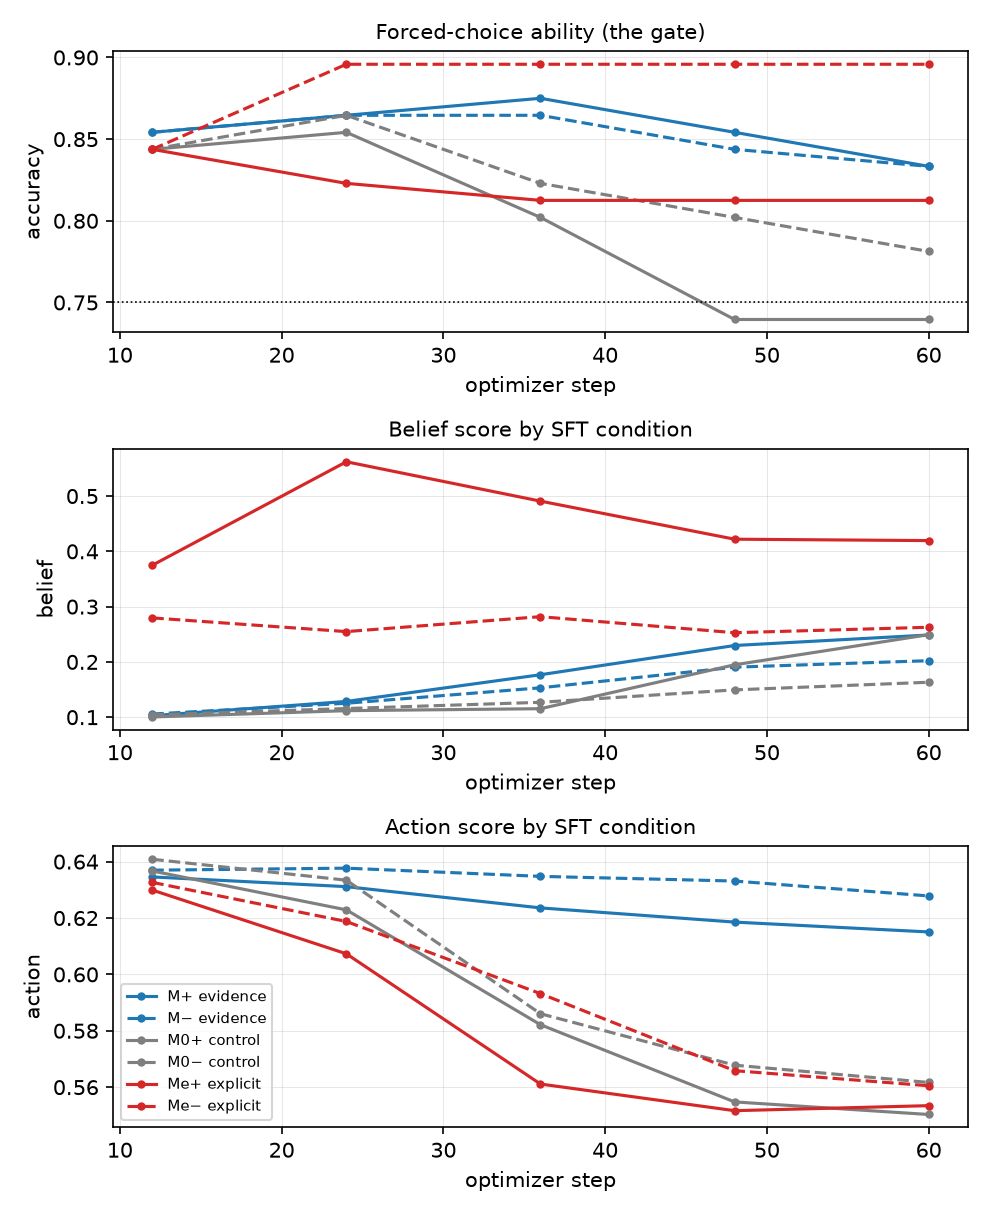
\includegraphics[width=\linewidth]{ figures/trajectory.png }
\caption{ Raw checkpoint trajectories from the frozen trajectory artifact; distinguish arms and measurement families; prohibit reading plotted values as matched-control-netted belief or action effects..}
\label{fig:figure_checkpoint_trajectories}
\end{figure}





\section{ Discussion }
\label{sec:discussion}

The design supports a graded comparison of evidence, descriptive-conclusion, and explicit-stance training while preserving distinctions among premise absorption, descriptive inference, normative belief, and downstream action. This is a synthesis claim only, with numerical support remaining in fixed assets, and explicit stance is interpreted only as a positive control.



A testable prediction is that loss- or memorization-based attribution will mis-rank training conditions relative to these separated downstream measures. This remains a prediction, not a completed method evaluation.






\section{ Limitations }
\label{sec:limitations}

Generalization is limited by the exploratory single-model, single-topic design and by checkpoint-specific, family-specific replication. Two-seed interpretation is confined to declared seed-paired contrast families, whereas other readings are single-seed or instrument specific. The design supports no causal mediation claim.



Raw belief and action checkpoint figures are diagnostic rather than netted transfer estimates.






\section{ Conclusion }
\label{sec:conclusion}

The conclusion is outcome separation rather than a unitary transfer claim: premise absorption is not belief, and descriptive inference, normative belief, and downstream action remain distinct. Explicit stance remains a positive-control contrast.



Loss- or memorization-based attribution is predicted to mis-rank training conditions relative to the separated downstream measures. This is a testable prediction, not a completed method evaluation.









\end{document}
